\documentclass{article}

\usepackage[utf8] {inputenc}
\usepackage {graphicx}
\usepackage {MnSymbol}
\usepackage {tikz}
\usepackage {media9}
\usetikzlibrary {arrows, shapes}
\usepackage {stmaryrd}
\usepackage {colortbl}
\usepackage {caption}
\usepackage {comment}
\usepackage {pdfpages}
\usepackage {listings}
\usepackage {color}
\usepackage {booktabs}
\usepackage {soul}
\usepackage[normalem] {ulem}

\usepackage {tcolorbox}
\usepackage {lipsum}
\usepackage {pgf}
\usepackage {etex}
\usepackage {tikz, pgfplots}

\tikzstyle {every picture} +  = [remember picture]
\everymath {\displaystyle}

\usepackage[square, numbers] {natbib} % \bibliographystyle {unsrtnat}

\hypersetup {
colorlinks = true, 
linkcolor = blue, 
filecolor = magenta, 
urlcolor = cyan, 
}

\mode<presentation> {

% The Beamer class comes with a number of default slide themes
% which change the colors and layouts of slides. Below this is a list
% of all the themes, uncomment each in turn to see what they look like.

%\usetheme{default}
%\usetheme{AnnArbor}
%\usetheme{Antibes}
%\usetheme{Bergen}
%\usetheme{Berkeley}
%\usetheme{Berlin}
%\usetheme{Boadilla}
%\usetheme{CambridgeUS}
%\usetheme{Copenhagen}
%\usetheme{Darmstadt}
%\usetheme{Dresden}
%\usetheme{Frankfurt}
%\usetheme{Goettingen}
%\usetheme{Hannover}
%\usetheme{Ilmenau}
%\usetheme{JuanLesPins}
%\usetheme{Luebeck}
%\usetheme{Madrid}
\usetheme{Malmoe}
%\usetheme{Marburg}
%\usetheme{Montpellier}
%\usetheme{PaloAlto}
%\usetheme{Pittsburgh}
%\usetheme{Rochester}
%\usetheme{Singapore}
%\usetheme{Szeged}
%\usetheme{Warsaw}

% As well as themes, the Beamer class has a number of color themes
% for any slide theme. Uncomment each of these in turn to see how it
% changes the colors of your current slide theme.

%\usecolortheme{albatross}
%\usecolortheme{beaver}
%\usecolortheme{beetle}
%\usecolortheme{crane}
%\usecolortheme{dolphin}
%\usecolortheme{dove}
%\usecolortheme{fly}
%\usecolortheme{lily}
%\usecolortheme{orchid}
%\usecolortheme{rose}
%\usecolortheme{seagull}
%\usecolortheme{seahorse}
\usecolortheme{whale}
%\usecolortheme{wolverine}

%\setbeamertemplate{footline} % To remove the footer line in all slides uncomment this line
% To replace the footer line in all slides with a simple slide count uncomment this line
\setbeamertemplate{footline}[page number]
% To remove the navigation symbols from the bottom of all slides uncomment this line
\setbeamertemplate{navigation symbols}{}
\usefonttheme {professionalfonts}
\useoutertheme {infolines}
\useinnertheme {circles}
}


\newtheorem *  {bem} {Bemerkung}

\usepackage {tikz}

\usepackage {listings}
\usepackage {color}

\definecolor {dkgreen} {rgb} {0, 0.6, 0}
\definecolor {gray} {rgb} {0.5, 0.5, 0.5}
\definecolor {mauve} {rgb} {0.58, 0, 0.82}

\lstset {frame = tb, 
language = Java, 
aboveskip = 2mm, 
belowskip = 12mm, 
showstringspaces = false, 
columns = flexible, 
basicstyle =  {\small\ttfamily}, 
numbers = none, 
numberstyle = \tiny\color {gray}, 
keywordstyle = \color {blue}, 
commentstyle = \color {dkgreen}, 
stringstyle = \color {mauve}, 
breaklines = true, 
breakatwhitespace = true, 
tabsize = 2
} % Include the file specifying the document structure and custom commands
\title{My Document}
\author{Ying Cao}
\date{\today}

\begin{document}
\bibliographystyle{plain}

\maketitle % Print the title
\tableofcontents

\noindent
\linespread{1.2}
\selectfont
\setlength{\topskip}{0ex}
\setlength{\parskip}{1ex}
\setlength{\lineskip}{1em}

%---------------------------------------------------------------
% unnumbered section
%---------------------------------------------------------------

\section{Introduction}

This is the introduction. 

Paper \cite{lamport1974parallel} studies the compilation techniques for a kind of loop program transformation
targeting multiprocessor computers.

\begin{figure}[ht]
  \centering
  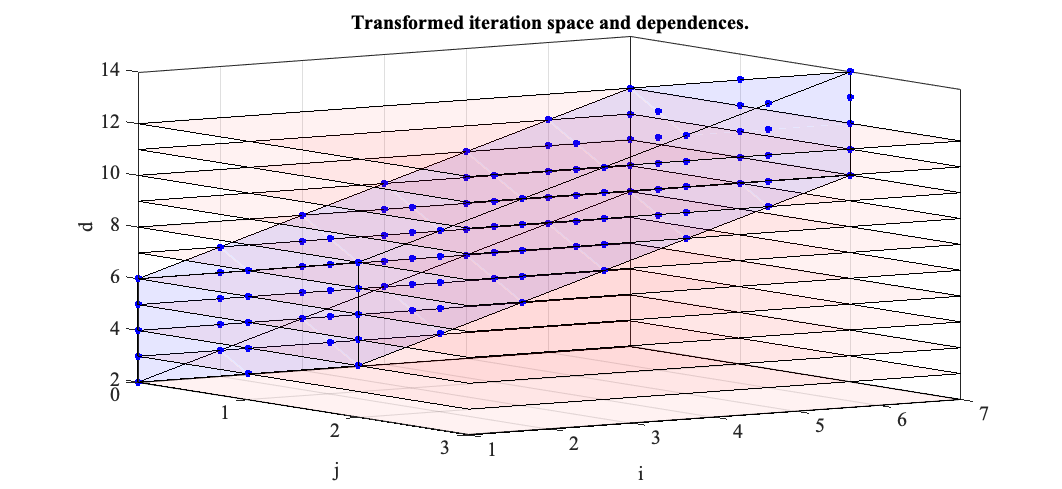
\includegraphics[scale=0.4]{figures/figure1.png}
  \caption{this is a figure demo}
  \label{fig:label}
\end{figure}

% Math equation/formula
\begin{equation}
I = \int_{a}^{b} f(x) \; \text{d}x.
\end{equation}

\begin{info} % Information block
This is an interesting piece of information, to which the reader should pay special attention.
\end{info}

\section{Section title} % Numbered section

This is the numbered section.

\subsection{Subsection title}

This is the numbered sub section.

%------------------------------------------------------------------
% Numbered question, with subquestions in an enumerate environment
%------------------------------------------------------------------
\begin{question}
    This is a question.

  % Subquestions numbered with letters
  \begin{enumerate}[(a)]
    \item Do this.
    \item Do that.
    \item Do something else.
  \end{enumerate}
\end{question}

%------------------------------------------------------------------
% Algorithm
%------------------------------------------------------------------
\subsection{Algorithmic issues}


\begin{center}
  \begin{minipage}{0.5\linewidth} % Adjust the minipage width to accomodate for the length of algorithm lines
    \begin{algorithm}[H]
      \KwIn{$(a, b)$, two floating-point numbers}  % Algorithm inputs
      \KwResult{$(c, d)$, such that $a+b = c + d$} % Algorithm outputs/results
      \medskip
      \If{$\vert b\vert > \vert a\vert$}{
          exchange $a$ and $b$ \;
      }
      $c \leftarrow a + b$ \;
      $z \leftarrow c - a$ \;
      $d \leftarrow b - z$ \;
      {\bf return} $(c,d)$ \;
      \caption{\texttt{FastTwoSum}} % Algorithm name
      \label{alg:fastTwoSum}   % optional label to refer to
    \end{algorithm}
  \end{minipage}
\end{center}

Descriptions of the algorithm.

%------------------------------------------------------------------
% Numbered question, with an optional title
%------------------------------------------------------------------
\begin{question}[\itshape (with optional title)]
    Describe your question.
\end{question}

Desciptions.

\section{Implementation}

Describe your implementation here.

% code snippets.
\begin{lstlisting}[language=Python]
#! /usr/bin/python

import sys
sys.stdout.write("Hello World!\n")
\end{lstlisting}

Explanations of the implementation.

\bibliography{references.bib}
\end{document}
